
%  Multigrid FSP for the RDME
%  Aditya Dendukuri

\documentclass[10pt,aspectratio=169]{beamer}

\usetheme{Boadilla}
\usecolortheme{seahorse}
\setbeamertemplate{navigation symbols}{}
\setbeamerfont{frametitle}{size=\normalsize,series=\bfseries}
\setbeamerfont{title}{size=\large,series=\bfseries}
\setbeamertemplate{bibliography item}[text]

\usepackage{amsmath,amssymb,bm,mathtools}
\usepackage{tikz}
\usetikzlibrary{arrows.meta,positioning,patterns,decorations.pathreplacing,calc}
\usepackage{graphicx}
\usepackage{booktabs}
\usepackage{xcolor}
\usepackage{pifont}

\graphicspath{{figures/}}

\newcommand{\Bin}{\operatorname{Bin}}
\newcommand{\calR}{\mathcal{R}}
\newcommand{\calP}{\mathcal{P}}
\newcommand{\citeref}[1]{{\scriptsize\textcolor{gray}{[#1]}}}

\definecolor{fastblue}{RGB}{31,119,180}
\definecolor{slowred}{RGB}{214,39,40}
\definecolor{coarsegreen}{RGB}{44,160,44}
\definecolor{coarsecolor}{RGB}{31,119,180}
\definecolor{intercolor}{RGB}{255,140,0}
\definecolor{myblue}{RGB}{31,119,180}
\definecolor{mygray}{RGB}{80,80,80}

\title[Multigrid FSP for RDME]{%
  Multigrid Finite State Projection\\
  for the Reaction-Diffusion Master Equation}
\author{Aditya Dendukuri}
\institute[UCSB]{University of California, Santa Barbara}
\date{}

\begin{document}

\begin{frame}\titlepage\end{frame}

%================================================================
%  1. THE RDME
%================================================================

\begin{frame}{The RDME: reactions and diffusion across a spatial grid}

  \begin{columns}[T]
    \begin{column}{0.50\textwidth}
      \textbf{Model.}
      Divide a 1-D domain into $K$ voxels.
      Each voxel $k$ holds molecule counts $\mathbf{n}_k \in \mathbb{Z}_{\geq 0}^S$.

      \medskip
      Two types of events:
      \begin{itemize}\setlength\itemsep{0.4em}
        \item \textcolor{slowred}{\textbf{Reactions}} inside voxel $k$:
              rate $\alpha_r(\mathbf{n}_k)$, change $\mathbf{n}_k$.
        \item \textcolor{fastblue}{\textbf{Diffusion}} between neighbors:
              rate $d = D/h^2$, moves one molecule $k \leftrightarrow k{+}1$.
      \end{itemize}

      \medskip
      The joint probability $p(\mathbf{n}_1,\ldots,\mathbf{n}_K,t)$
      satisfies $\dot p = A p$ \textbf{(RDME)}.

      \medskip
      \begin{alertblock}{The computational bottleneck}
        The state space has $\sim n_{\max}^{SK}$ reachable states —
        \textbf{exponential in $K$}.
        Even $K{=}8$, $S{=}1$ is intractable with a naive FSP.
      \end{alertblock}
    \end{column}
    \begin{column}{0.46\textwidth}
      \begin{center}
      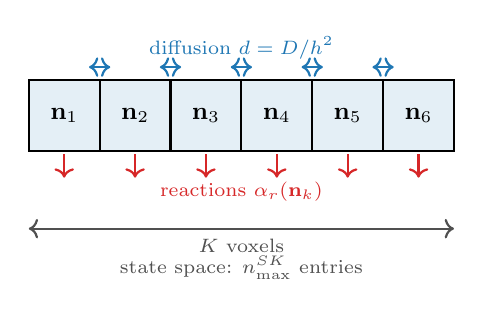
\begin{tikzpicture}[scale=0.90, every node/.style={font=\small}]
        \foreach \k in {1,2,3,4,5,6} {
          \draw[thick,fill=myblue!12] (\k-1,0) rectangle (\k,1.0);
          \node at (\k-0.5, 0.50) {$\mathbf{n}_\k$};
        }
        \foreach \k in {1,2,3,4,5} {
          \draw[<->,fastblue,thick] (\k-0.15,1.18) -- (\k+0.15,1.18);
        }
        \node[fastblue, font=\scriptsize] at (3, 1.45) {diffusion $d = D/h^2$};
        \foreach \k in {1,2,3,4,5,6} {
          \draw[->,slowred,thick] (\k-0.5,-0.05) -- (\k-0.5,-0.38);
        }
        \node[slowred, font=\scriptsize] at (3, -0.58) {reactions $\alpha_r(\mathbf{n}_k)$};
        \draw[<->,thick,mygray] (0,-1.1) -- (6,-1.1)
          node[midway,below,font=\scriptsize]{$K$ voxels};
        \node[mygray,font=\scriptsize] at (3,-1.65)
          {state space: $n_{\max}^{SK}$ entries};
      \end{tikzpicture}
      \end{center}
    \end{column}
  \end{columns}

\end{frame}

%================================================================
%  2. BLOCK-TRIDIAGONAL STRUCTURE
%================================================================

\begin{frame}{$\dot{p} = Ap$ has block-tridiagonal structure \textnormal{\small(schematic, $K{=}4$, $S{=}1$)}}

\vspace{-0.2cm}
\begin{center}
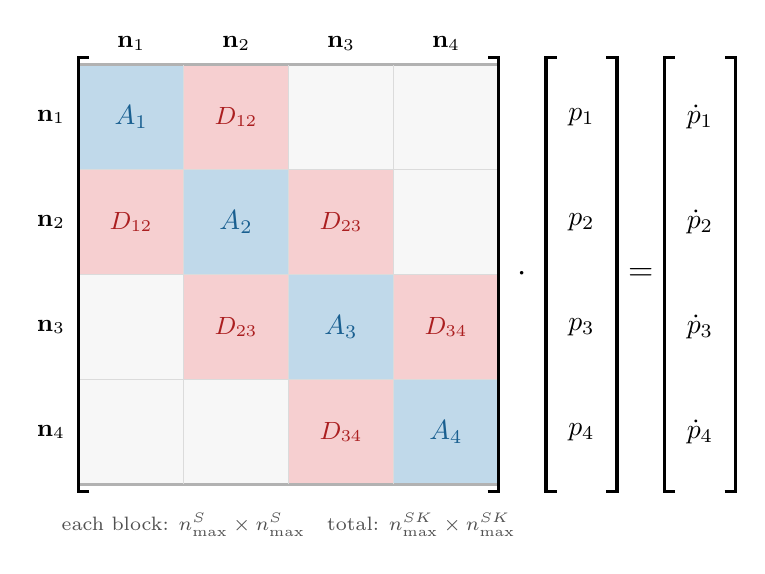
\begin{tikzpicture}[scale=0.86]
  \def\bs{1.55}
  \def\bw{0.16}
  \def\bp{0.10}

  \fill[gray!6] (0,0) rectangle (4*\bs,4*\bs);
  \foreach \k in {0,1,2,3}
    \fill[myblue!28] (\k*\bs,{(3-\k)*\bs}) rectangle ({(\k+1)*\bs},{(4-\k)*\bs});
  \foreach \k in {0,1,2} {
    \fill[slowred!22] ({(\k+1)*\bs},{(3-\k)*\bs}) rectangle ({(\k+2)*\bs},{(4-\k)*\bs});
    \fill[slowred!22] ({\k*\bs},{(2-\k)*\bs}) rectangle ({(\k+1)*\bs},{(3-\k)*\bs});
  }
  \draw[black!30,thick] (0,0) rectangle (4*\bs,4*\bs);
  \foreach \k in {1,2,3} {
    \draw[black!14,thin] (\k*\bs,0) -- (\k*\bs,4*\bs);
    \draw[black!14,thin] (0,\k*\bs) -- (4*\bs,\k*\bs);
  }
  \foreach \k/\l in {0/1,1/2,2/3,3/4}
    \node[font=\normalsize, myblue!80!black]
      at ({(\k+0.5)*\bs},{(3.5-\k)*\bs}) {$A_\l$};
  \node[font=\small,slowred!80!black] at (1.5*\bs,3.5*\bs) {$D_{12}$};
  \node[font=\small,slowred!80!black] at (0.5*\bs,2.5*\bs) {$D_{12}$};
  \node[font=\small,slowred!80!black] at (2.5*\bs,2.5*\bs) {$D_{23}$};
  \node[font=\small,slowred!80!black] at (1.5*\bs,1.5*\bs) {$D_{23}$};
  \node[font=\small,slowred!80!black] at (3.5*\bs,1.5*\bs) {$D_{34}$};
  \node[font=\small,slowred!80!black] at (2.5*\bs,0.5*\bs) {$D_{34}$};
  \foreach \k/\l in {0/$\mathbf{n}_1$,1/$\mathbf{n}_2$,2/$\mathbf{n}_3$,3/$\mathbf{n}_4$} {
    \node[above,font=\small] at ({(\k+0.5)*\bs}, 4*\bs+0.06) {\l};
    \node[left, font=\small] at (-0.06, {(3.5-\k)*\bs}) {\l};
  }
  \draw[very thick]
    (\bw,-\bp) -- (0,-\bp) -- (0,4*\bs+\bp) -- (\bw,4*\bs+\bp);
  \draw[very thick]
    (4*\bs-\bw,-\bp) -- (4*\bs,-\bp) -- (4*\bs,4*\bs+\bp) -- (4*\bs-\bw,4*\bs+\bp);
  \def\vgap{0.70}
  \def\vw{1.05}
  \pgfmathsetmacro{\vx}{4*\bs + \vgap}
  \node[font=\large] at ({4*\bs + \vgap/2}, {2*\bs}) {$\cdot$};
  \draw[very thick]
    (\vx+\bw,-\bp) -- (\vx,-\bp) -- (\vx,4*\bs+\bp) -- (\vx+\bw,4*\bs+\bp);
  \draw[very thick]
    (\vx+\vw-\bw,-\bp) -- (\vx+\vw,-\bp) -- (\vx+\vw,4*\bs+\bp)
    -- (\vx+\vw-\bw,4*\bs+\bp);
  \foreach \k/\l in {0/$p_1$,1/$p_2$,2/$p_3$,3/$p_4$}
    \node[font=\normalsize] at (\vx+\vw/2, {(3.5-\k)*\bs}) {\l};
  \pgfmathsetmacro{\eqx}{\vx + \vw + \vgap/2}
  \node[font=\large] at (\eqx, {2*\bs}) {$=$};
  \pgfmathsetmacro{\rx}{\vx + \vw + \vgap}
  \draw[very thick]
    (\rx+\bw,-\bp) -- (\rx,-\bp) -- (\rx,4*\bs+\bp) -- (\rx+\bw,4*\bs+\bp);
  \draw[very thick]
    (\rx+\vw-\bw,-\bp) -- (\rx+\vw,-\bp) -- (\rx+\vw,4*\bs+\bp)
    -- (\rx+\vw-\bw,4*\bs+\bp);
  \foreach \k/\l in {0/$\dot p_1$,1/$\dot p_2$,2/$\dot p_3$,3/$\dot p_4$}
    \node[font=\normalsize] at (\rx+\vw/2, {(3.5-\k)*\bs}) {\l};
  \node[mygray,font=\scriptsize,below] at (2*\bs,-\bp-0.18)
    {each block: $n_{\max}^S \times n_{\max}^S$\quad total: $n_{\max}^{SK} \times n_{\max}^{SK}$};
\end{tikzpicture}
\end{center}

\vspace{0.3em}
{\small
  \textcolor{myblue!80!black}{$A_k$}: reactions inside voxel $k$
  \hspace{1.5em}
  \textcolor{slowred!80!black}{$D_{k,k+1}$}: diffusion between neighboring voxels
  \hspace{1.5em}
  $p_k$: probability sub-vector for voxel $k$
}

\end{frame}

%================================================================
%  3. BINOMIAL IS EXACT DIFFUSION EQUILIBRIUM
%================================================================

\begin{frame}{The Binomial is the exact diffusion equilibrium}

  \begin{columns}[T]
    \begin{column}{0.50\textwidth}
      \textbf{Fix total molecules} $\bar n = n_1 + n_2$ across two adjacent voxels.

      \smallskip
      Diffusion moves one molecule at a time, at rate $d$ per molecule:

      \begin{center}
      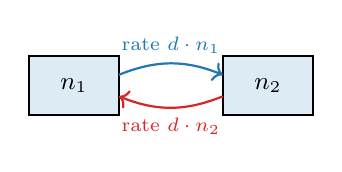
\begin{tikzpicture}[every node/.style={font=\small}, scale=0.88]
        \draw[thick,fill=coarsecolor!15] (0,0) rectangle (1.3,0.85);
        \draw[thick,fill=coarsecolor!15] (2.8,0) rectangle (4.1,0.85);
        \node at (0.65, 0.42) {$n_1$};
        \node at (3.45, 0.42) {$n_2$};
        \draw[->,fastblue,thick,bend left=22] (1.3,0.58)
          to node[above,font=\scriptsize]{rate $d\cdot n_1$} (2.8,0.58);
        \draw[->,slowred,thick,bend left=22]  (2.8,0.27)
          to node[below,font=\scriptsize]{rate $d\cdot n_2$} (1.3,0.27);
      \end{tikzpicture}
      \end{center}

      Each molecule hops independently $\Rightarrow$ at equilibrium, equally
      likely to be in either voxel. For $\bar n$ total:
      \[
        \boxed{P(n_1 \mid \bar n) = \Bin\!\bigl(\bar n,\,\tfrac{1}{2}\bigr)}
        \quad \text{(exact, any } d > 0\text{)}
      \]
      When the distribution is near this equilibrium,
      \textbf{$\bar n$ alone describes the two-voxel state}.
    \end{column}
    \begin{column}{0.46\textwidth}
      \begin{center}
      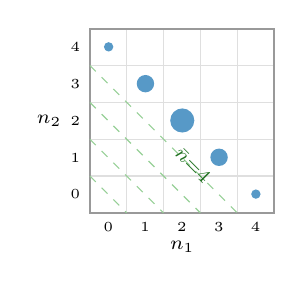
\begin{tikzpicture}[scale=0.85]
        \def\cs{0.55}
        \draw[gray!25](0,0) grid[step=\cs] (5*\cs,5*\cs);
        \draw[black!40,thick](0,0) rectangle (5*\cs,5*\cs);
        \foreach \t in {1,2,3,4} {
          \draw[coarsegreen!50,dashed,thin]
            ({max(0,\t-4)*\cs},{min(\t,4)*\cs}) -- ({min(\t,4)*\cs},{max(0,\t-4)*\cs});
        }
        \fill[coarsecolor!75](0.28,2.48) circle (0.07cm);
        \fill[coarsecolor!75](0.83,1.93) circle (0.13cm);
        \fill[coarsecolor!75](1.38,1.38) circle (0.18cm);
        \fill[coarsecolor!75](1.93,0.83) circle (0.13cm);
        \fill[coarsecolor!75](2.48,0.28) circle (0.07cm);
        \foreach \n in {0,1,2,3,4}
          \node[below,font=\tiny] at ({(\n+0.5)*\cs},0) {\n};
        \foreach \n in {0,1,2,3,4}
          \node[left,font=\tiny]  at (0,{(\n+0.5)*\cs}) {\n};
        \node[below,font=\scriptsize] at (1.38,-0.28) {$n_1$};
        \node[left, font=\scriptsize] at (-0.28,1.38) {$n_2$};
        \node[coarsegreen!70!black,font=\scriptsize,rotate=-45] at (2.8*\cs,1.3*\cs) {$\bar n{=}4$};
      \end{tikzpicture}

      \vspace{0.4em}
      {\footnotesize
        Probability spreads along constant-total diagonals
        as $\Bin(\bar n,\tfrac12)$ (dot size $\propto$ mass).\\[0.3em]
        \textbf{The two-voxel state is captured by $\bar n$ alone.}
      }
      \end{center}
    \end{column}
  \end{columns}

\end{frame}

%================================================================
%  4. MERGING: R AND P OPERATORS
%================================================================

\begin{frame}{Merging two adjacent voxels: restriction and prolongation}

  \begin{columns}[T]
    \begin{column}{0.50\textwidth}
      \textbf{Compress ($\calR$): exact:}
      \[ p^c(\bar n) = \!\!\sum_{n_1 + n_2 = \bar n}\!\! p(n_1, n_2). \]

      \textbf{Reconstruct ($\calP$): approximate:}
      \[ p(n_1, n_2) \approx p^c(\bar n)\cdot\Bin(\bar n,\tfrac{1}{2}). \]

      \begin{block}{State-space reduction}
        Per pair: $n_{\max}^{2S} \to n_{\max}^{S}$.\\
        All $K$ voxels: $n_{\max}^{SK} \to n_{\max}^{SK/2}$.
      \end{block}

      \smallskip
      {\small $\calP$ is accurate when the distribution is near-Binomial
     : verified at runtime, not assumed globally.}
    \end{column}
    \begin{column}{0.46\textwidth}
      \begin{center}
      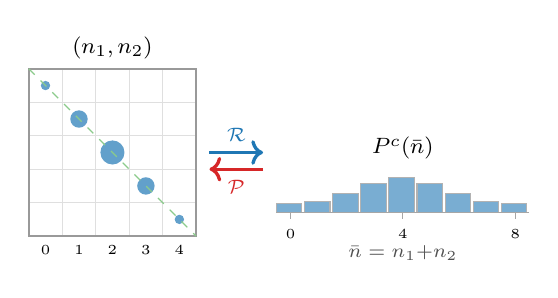
\begin{tikzpicture}[scale=0.85, every node/.style={font=\scriptsize}]
        \def\cs{0.50}
        \draw[gray!25](0,0) grid[step=\cs] (5*\cs,5*\cs);
        \draw[black!40,thick](0,0) rectangle (5*\cs,5*\cs);
        \node[above,font=\footnotesize] at (1.25,2.5) {$(n_1,n_2)$};
        \fill[coarsecolor!70](0.25,2.25) circle (0.07cm);
        \fill[coarsecolor!70](0.75,1.75) circle (0.13cm);
        \fill[coarsecolor!70](1.25,1.25) circle (0.18cm);
        \fill[coarsecolor!70](1.75,0.75) circle (0.13cm);
        \fill[coarsecolor!70](2.25,0.25) circle (0.07cm);
        \draw[coarsegreen!55,dashed](0,2.5)--(2.5,0);
        \foreach \n in {0,1,2,3,4}
          \node[below,font=\tiny] at ({(\n+0.5)*\cs},0) {\n};
        \draw[->,very thick,coarsecolor] (2.7,1.25) -- (3.5,1.25)
          node[above,midway,font=\scriptsize]{$\calR$};
        \draw[->,very thick,slowred]     (3.5,1.0)  -- (2.7,1.0)
          node[below,midway,font=\scriptsize]{$\calP$};
        \def\cb{0.42}
        \foreach \nb in {0,1,2,3,4,5,6,7,8} {
          \pgfmathsetmacro{\ht}{0.12 + 0.40*exp(-0.5*((\nb-4)/1.5)*((\nb-4)/1.5))}
          \fill[coarsecolor!60] (3.7+\nb*\cb, 0.35) rectangle
                                (3.7+\nb*\cb+\cb-0.04, 0.35+\ht);
          \draw[black!30] (3.7+\nb*\cb, 0.35) rectangle
                          (3.7+\nb*\cb+\cb-0.04, 0.35+\ht);
        }
        % x-axis labels
        \draw[black!35] (3.7,0.35) -- (3.7+9*\cb,0.35);
        \foreach \nb/\lbl in {0/0, 4/4, 8/8} {
          \draw[black!35] (3.7+\nb*\cb+\cb/2,0.35) -- (3.7+\nb*\cb+\cb/2,0.25);
          \node[below,font=\tiny] at (3.7+\nb*\cb+\cb/2,0.25) {\lbl};
        }
        \node[below,font=\scriptsize,mygray] at (3.7+4.5*\cb,0.0)
          {$\bar n = n_1{+}n_2$};
        \node[above,font=\footnotesize] at (3.7+4*\cb+\cb/2, 1.0) {$P^c(\bar n)$};
      \end{tikzpicture}

      \vspace{0.3em}
      {\footnotesize
        $\calR$: sum along each diagonal $\to$ scalar $\bar n = n_1{+}n_2$.\\
        $\calP$: spread back via $\Bin(\bar n, \tfrac{1}{2})$.
      }
      \end{center}
    \end{column}
  \end{columns}

\end{frame}

%================================================================
%  5. WHAT MERGING DOES TO THE RATE MATRIX
%================================================================

\begin{frame}{What merging does to the rate matrix}

  \begin{columns}[T]
    \begin{column}{0.44\textwidth}
      \textbf{Full matrix $A$: 4 voxels:}
      \begin{center}
      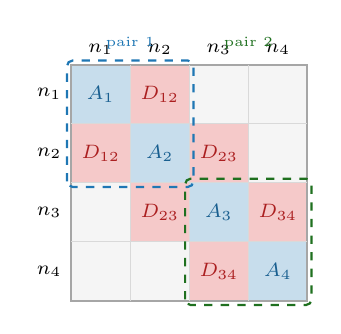
\begin{tikzpicture}[scale=0.75]
        \def\bs{1.00}
        \fill[gray!8] (0,0) rectangle (4*\bs,4*\bs);
        \foreach \k in {0,...,3}
          \fill[myblue!25] (\k*\bs,{(3-\k)*\bs}) rectangle ({(\k+1)*\bs},{(4-\k)*\bs});
        \foreach \k/\kp in {0/1,1/2,2/3} {
          \fill[slowred!25] (\kp*\bs,{(3-\k)*\bs}) rectangle ({(\kp+1)*\bs},{(4-\k)*\bs});
          \fill[slowred!25] (\k*\bs,{(3-\kp)*\bs}) rectangle ({(\k+1)*\bs},{(4-\kp)*\bs});
        }
        \draw[black!35,thick] (0,0) rectangle (4*\bs,4*\bs);
        \foreach \k in {1,...,3} {
          \draw[black!15,thin] (\k*\bs,0) -- (\k*\bs,4*\bs);
          \draw[black!15,thin] (0,\k*\bs) -- (4*\bs,\k*\bs);
        }
        \foreach \k/\l in {0/1,1/2,2/3,3/4}
          \node[font=\scriptsize,myblue!80!black]
            at ({(\k+0.5)*\bs},{(3.5-\k)*\bs}) {$A_\l$};
        \node[font=\scriptsize,slowred!80!black] at (1.5*\bs,3.5*\bs) {$D_{12}$};
        \node[font=\scriptsize,slowred!80!black] at (0.5*\bs,2.5*\bs) {$D_{12}$};
        \node[font=\scriptsize,slowred!80!black] at (2.5*\bs,2.5*\bs) {$D_{23}$};
        \node[font=\scriptsize,slowred!80!black] at (1.5*\bs,1.5*\bs) {$D_{23}$};
        \node[font=\scriptsize,slowred!80!black] at (3.5*\bs,1.5*\bs) {$D_{34}$};
        \node[font=\scriptsize,slowred!80!black] at (2.5*\bs,0.5*\bs) {$D_{34}$};
        \foreach \k/\l in {0/$n_1$,1/$n_2$,2/$n_3$,3/$n_4$} {
          \node[above,font=\scriptsize] at ({(\k+0.5)*\bs},4*\bs) {\l};
          \node[left, font=\scriptsize] at (0,{(3.5-\k)*\bs}) {\l};
        }
        \draw[coarsecolor,thick,dashed,rounded corners=2pt]
          (-0.07,{2*\bs-0.07}) rectangle ({2*\bs+0.07},{4*\bs+0.07});
        \draw[coarsegreen!70!black,thick,dashed,rounded corners=2pt]
          ({2*\bs-0.07},{-0.07}) rectangle ({4*\bs+0.07},{2*\bs+0.07});
        \node[coarsecolor,font=\tiny,above] at (\bs,4*\bs+0.1) {pair 1};
        \node[coarsegreen!70!black,font=\tiny,above] at (3*\bs,4*\bs+0.1) {pair 2};
      \end{tikzpicture}
      \end{center}
      {\footnotesize Size: $n_{\max}^4$}
    \end{column}
    \begin{column}{0.10\textwidth}
      \vspace{2.6cm}
      \begin{center}
        $\xrightarrow{\;\calR\;}$\\[0.5em]
        $\xleftarrow{\;\calP\;}$
      \end{center}
    \end{column}
    \begin{column}{0.42\textwidth}
      \textbf{Merged matrix $\bar A$: 2 pairs:}
      \begin{center}
      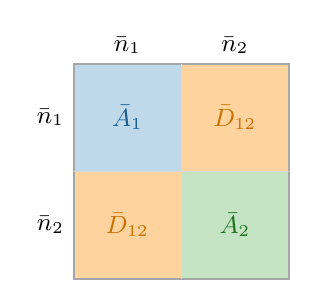
\begin{tikzpicture}[scale=0.75]
        \def\cs{1.82}
        \fill[gray!8] (0,0) rectangle (2*\cs,2*\cs);
        \fill[coarsecolor!28]  (0,\cs) rectangle (\cs,2*\cs);
        \fill[coarsegreen!28]  (\cs,0) rectangle (2*\cs,\cs);
        \fill[intercolor!38] (0,0) rectangle (\cs,\cs);
        \fill[intercolor!38] (\cs,\cs) rectangle (2*\cs,2*\cs);
        \draw[black!35,thick] (0,0) rectangle (2*\cs,2*\cs);
        \draw[black!15,thin] (\cs,0) -- (\cs,2*\cs);
        \draw[black!15,thin] (0,\cs) -- (2*\cs,\cs);
        \node[font=\small,coarsecolor!80!black]  at (0.5*\cs,1.5*\cs) {$\bar A_1$};
        \node[font=\small,coarsegreen!70!black]  at (1.5*\cs,0.5*\cs) {$\bar A_2$};
        \node[font=\small,intercolor!80!black]   at (0.5*\cs,0.5*\cs) {$\bar D_{12}$};
        \node[font=\small,intercolor!80!black]   at (1.5*\cs,1.5*\cs) {$\bar D_{12}$};
        \node[above,font=\small] at (0.5*\cs,2*\cs) {$\bar n_1$};
        \node[above,font=\small] at (1.5*\cs,2*\cs) {$\bar n_2$};
        \node[left, font=\small] at (0,1.5*\cs) {$\bar n_1$};
        \node[left, font=\small] at (0,0.5*\cs) {$\bar n_2$};
      \end{tikzpicture}
      \end{center}
      {\footnotesize Size: $n_{\max}^2$ \quad ($\mathbf{10^4\times}$ smaller for $n_{\max}{=}100$)}
      \begin{itemize}\setlength\itemsep{0.15em}
        \item $A_k \to \bar A_j$: reactions averaged over Binomial
        \item Within-pair $D$ disappears: implicit in Binomial
        \item $\bar D_{12}$: only between-pair diffusion remains
      \end{itemize}
    \end{column}
  \end{columns}

\end{frame}

%================================================================
%  ALGORITHM PSEUDOCODE
%================================================================

\begin{frame}{The multigrid FSP algorithm}

\begin{columns}[T]
\column{0.54\textwidth}

\textbf{\texttt{multigrid\_fsp}($u_0$, $T$, $\Delta t$)}\\[0.4em]

\begin{enumerate}\setlength\itemsep{0.25em}
  \item \textbf{Initialise}: $p \leftarrow \delta_{u_0}$;\; expand $\mathcal{S}$ by one shell

  \item \textbf{Detect front}:
    \[ \alpha_j = \frac{|\mu_{2j-1} - \mu_{2j}|}{\mu_{2j-1}+\mu_{2j}}, \quad
       j^* = \operatorname{argmax}_j\,\alpha_j \]
    Keep pairs $j^*\!\pm\!1$ fine; merge rest.

  \item \textbf{Restrict}: $\tilde n_j = n_{2j-1}+n_{2j}$ for merged pairs

  \item \textbf{Solve}: $p \leftarrow e^{\Delta t\,A^M}\,p$\quad (Krylov)

  \item \textbf{Prolong}: $\Bin(\tilde n_j,\tfrac12)$ for merged;
    dynamic-$\pi$ at fine pairs

  \item \textbf{Expand}: add one-step reachable states to $\mathcal{S}$

  \item \textbf{Prune}: remove $\{x : p(x) < \tau\}$

  \item Repeat from \textbf{2} until $t = T$
\end{enumerate}

\column{0.42\textwidth}
\vspace{0.5em}
\begin{block}{Cost per step}
  \textbf{Coarse solve}: $|\mathcal{S}^M| \ll N^K$\\
  \textbf{Expand}: $O(|\mathcal{S}^M| \cdot |\text{reactions}|)$\\
  \textbf{Prune}: $O(|\mathcal{S}^M|)$\\[0.4em]
  $\mathcal{S}^M$ tracks only the support of $p$: never the full truncated space.
\end{block}

\vspace{0.5em}
\begin{block}{Key decision (step 2)}
  $\alpha_j \approx 0$: merge pair $j$ (Binom exact)\\
  $\alpha_j \approx 1$: keep fine (front present)\\[0.3em]
  Same criterion for birth-death and Schl\"{o}gl.
\end{block}

\end{columns}

\end{frame}

%================================================================
%  6. ADAPTIVE FSP ALGORITHM
%================================================================

\begin{frame}{The adaptive FSP algorithm: expand, solve, prune}
\begin{center}
  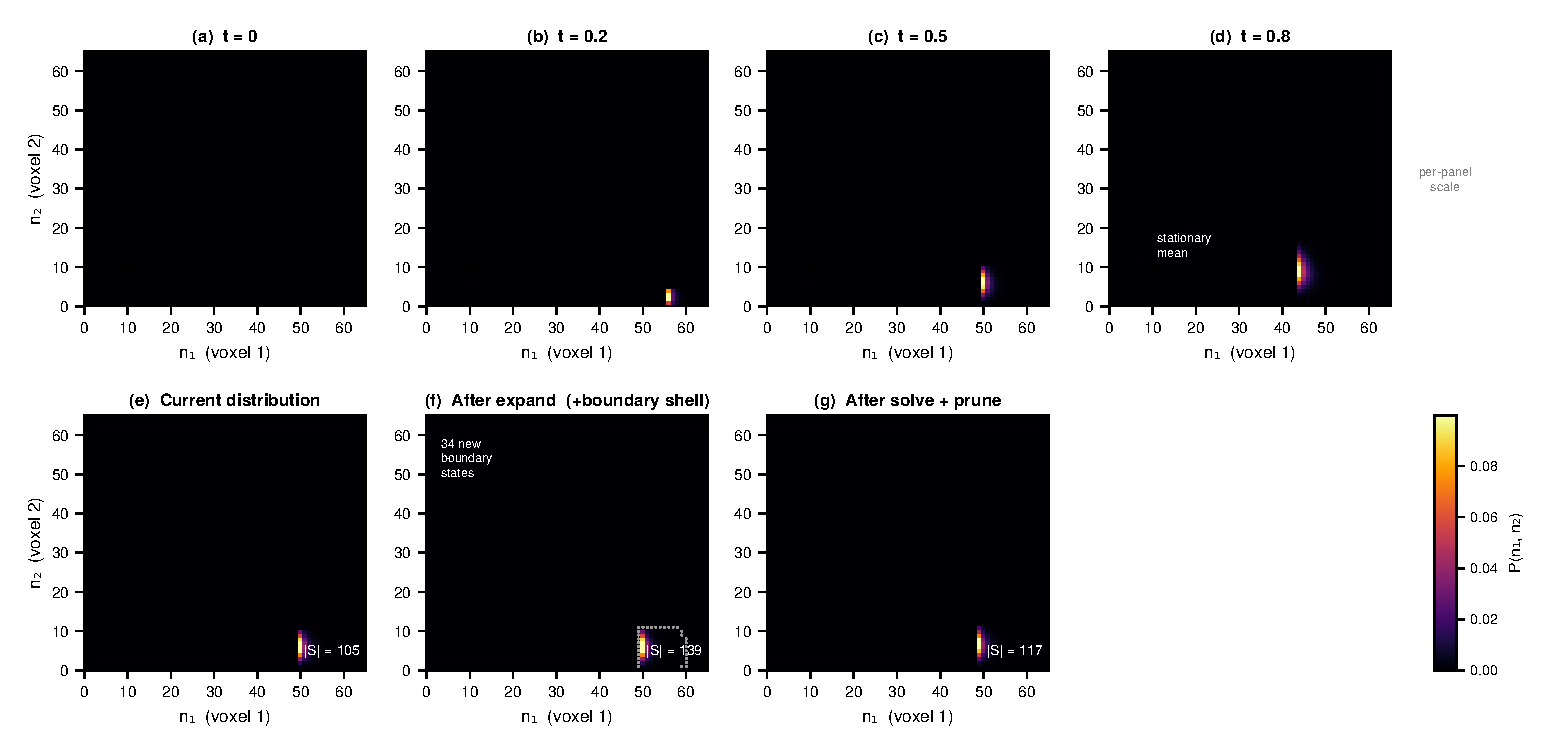
\includegraphics[width=0.92\textwidth,keepaspectratio]{fig_talk_fsp}
\end{center}
\vspace{-0.4em}
{\small
\textbf{Top row:} joint distribution $P(n_1,n_2)$ of a 2-voxel birth-death system: point source at $(n_\text{src},0)$ traveling to the stationary point (white cross).\\[0.2em]
\textbf{Bottom row} (one step at $t{=}0.5$):
\textbf{(e)}~Current support $|S|{=}105$.
\textbf{(f)}~After expand $|S|{=}139$: thin boundary shell added (white dots).
\textbf{(g)}~After solve+prune $|S|{=}117$: compact again.}
\end{frame}

%================================================================
%  7. BIRTH-DEATH RESULT
%================================================================

\begin{frame}{Result: K=8 RDME wavefront via coarsened simulation}
\begin{center}
  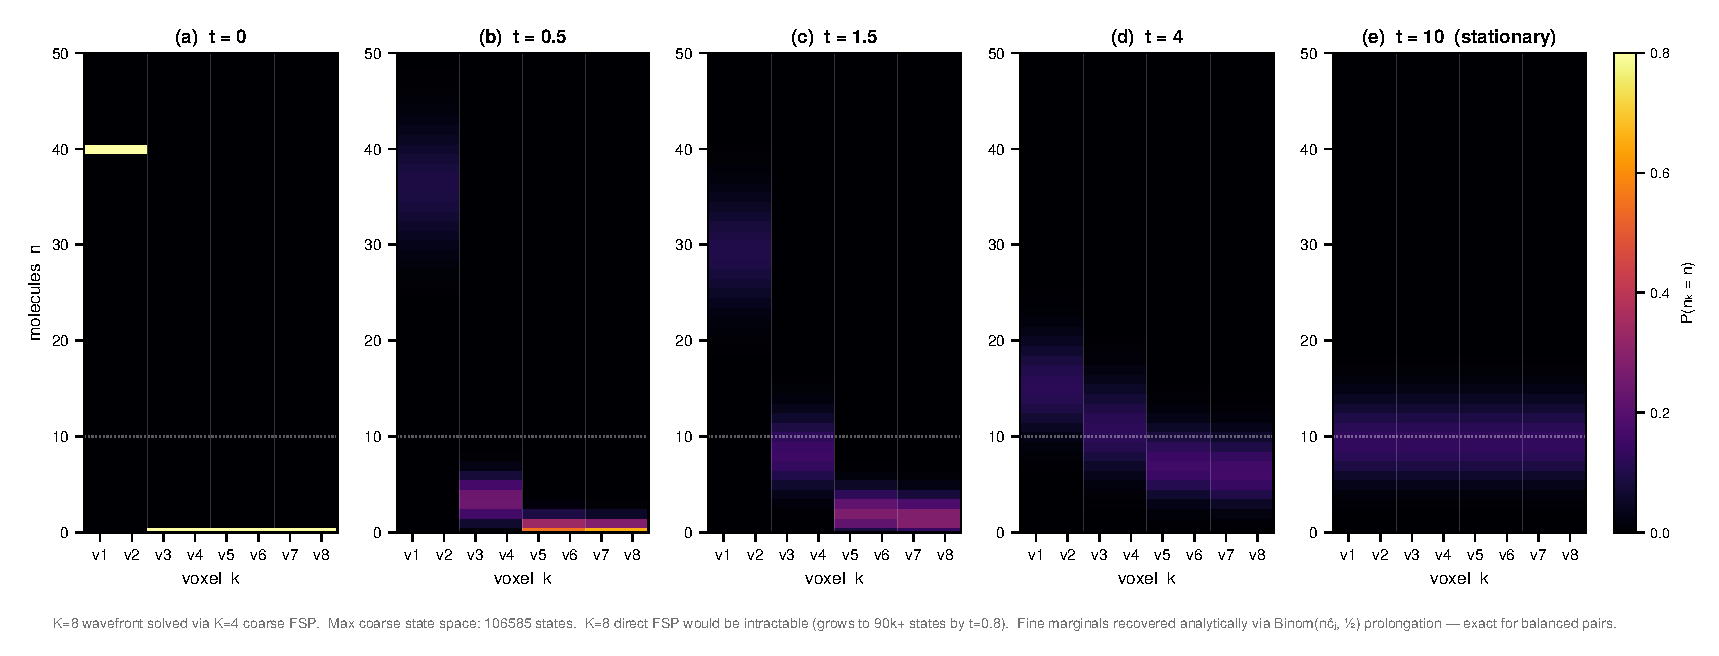
\includegraphics[width=0.92\textwidth,keepaspectratio]{fig_talk_result}
\end{center}
\vspace{-0.4em}
{\small
Birth-death RDME, $K{=}8$, $D{=}0.1$.
IC: $v_1{=}v_2{=}40$ (delta), $v_3\ldots v_8{=}0$.
Each panel shows marginals $P(n_k{=}n)$ for all 8 voxels.\\[0.2em]
\textbf{(a)--(d):} Wavefront sweeps left$\to$right, distributions broaden.
\textbf{(e):} Stationary: all voxels reach $\operatorname{Poisson}(10)$ (dashed line).\\[0.2em]
Solved via \textbf{K=4 coarse FSP} (30k states). Direct K=8 FSP: intractable.
Fine marginals recovered via $\operatorname{Bin}(\tilde{n},\tfrac12)$: \emph{exact} for balanced pairs.}
\end{frame}

%================================================================
%  TRANSITION TO BISTABILITY
%================================================================

\begin{frame}{What about bistable reactions?}

\begin{columns}[T]
\column{0.50\textwidth}
\textbf{Birth-death: coarsening is exact at stationarity.}\\[0.4em]
Each voxel has a single stable state.
Pairs equilibrate to $\Bin(\tilde{n},\tfrac12)$: merging always valid.

\vspace{0.8em}
\textbf{But what if reactions are bistable?}\\[0.4em]
Some systems have \emph{two} stable states per voxel.
Spatial fronts form where neighbors occupy opposite states.
These fronts are metastable: persistent for very long times.

\column{0.46\textwidth}
\vspace{0.3em}
\begin{block}{The Schl\"{o}gl model}
Bistable autocatalytic reactions:\\[0.3em]
\quad $\emptyset \rightleftharpoons X$ \quad (zeroth/first order)\\
\quad $2X \rightleftharpoons 3X$ \quad (auto-catalysis)\\[0.3em]
Two stable states: $n_\text{lo} \approx 31$ and $n_\text{hi} \approx 162$.\\[0.3em]
At a spatial front: joint $P(n_k,n_{k+1})$ is \emph{bimodal} —
Binomial prolongation is completely wrong.
\end{block}
\end{columns}

\end{frame}

%================================================================
%  8. BISTABILITY
%================================================================

\begin{frame}{Each voxel is bistable: two stable molecular states}
\begin{center}
  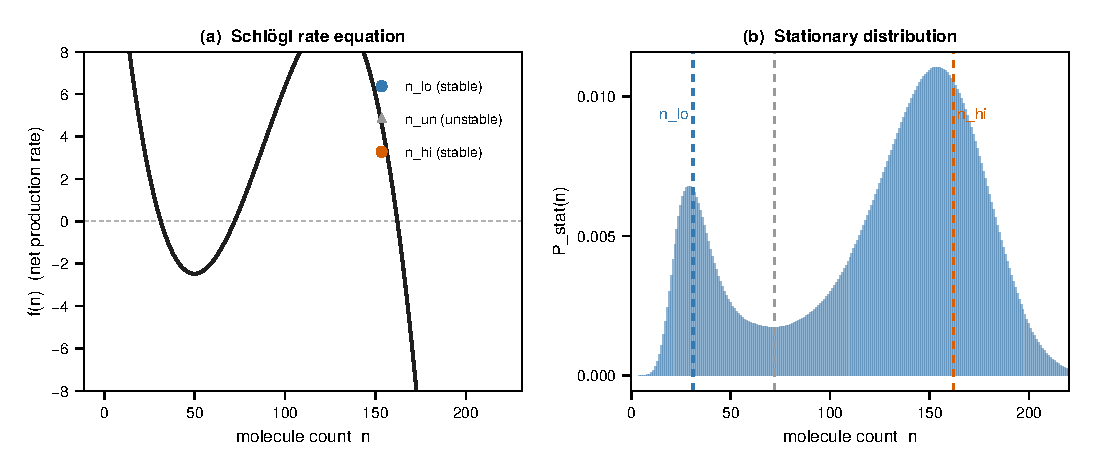
\includegraphics[width=0.86\textwidth,keepaspectratio]{fig_talk_bistability}
\end{center}
\vspace{-0.3em}
{\small
\textbf{(a)} Net production rate $f(n)$: three zeros: two stable ($n_\text{lo}$, $n_\text{hi}$), one unstable.
\quad\textbf{(b)} Stationary distribution is bimodal.\\[0.2em]
\emph{Think of it as a double-well potential: each voxel wants to be at $n_\text{lo}$ or $n_\text{hi}$.}
Each spatial configuration: e.g., $(n_\text{lo},n_\text{lo},n_\text{hi},n_\text{hi},\ldots)$: is metastable.}
\end{frame}

%================================================================
%  7. MERGING FAILS AT THE FRONT
%================================================================

\begin{frame}{Bistable fronts: when does Binomial coarsening fail?}

  \begin{columns}[T]
    \begin{column}{0.46\textwidth}
      \textbf{A spatial front} forms when neighboring voxels occupy opposite stable states.
      Slow diffusion sustains it indefinitely.

      \medskip
      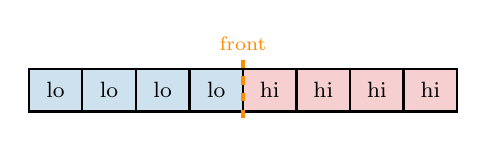
\begin{tikzpicture}[scale=0.68, every node/.style={font=\footnotesize}]
        \foreach \k in {1,2,3,4} {
          \draw[thick,fill=myblue!22] (\k-1,0) rectangle (\k,0.8);
          \node at (\k-0.5,0.4) {lo};
        }
        \foreach \k in {5,6,7,8} {
          \draw[thick,fill=slowred!22] (\k-1,0) rectangle (\k,0.8);
          \node at (\k-0.5,0.4) {hi};
        }
        \draw[very thick,intercolor,dashed] (4,-0.12) -- (4,0.96);
        \node[intercolor,above,font=\scriptsize] at (4,0.96) {front};
      \end{tikzpicture}

      \medskip
      At the interface pair: the joint $P(n_k,n_{k+1})$ is \textbf{bimodal}
      (two orientations: lo$|$hi and hi$|$lo).

      \vspace{0.5em}
      Coarsening sums $\tilde n = n_k + n_{k+1}$: both orientations give the \emph{same} total.
      Binomial prolongation puts both voxels at $\tilde n/2 \approx 97$.
      \textbf{Wrong.}

    \end{column}
    \begin{column}{0.50\textwidth}
      \vspace{0.3em}
      \begin{block}{The symmetry trap}
        \[
          (n_\text{lo},\,n_\text{hi}) \xrightarrow{\calR} \tilde n = 193
          \xleftarrow{\calR} (n_\text{hi},\,n_\text{lo})
        \]
        Both front orientations map to the same coarse state.
        $\calP$ cannot recover the orientation.
      \end{block}

      \vspace{0.4em}
      \begin{block}{Birth-death vs.\ Schl\"{o}gl}
        \begin{tabular}{@{}lcc@{}}
          & BD & Schl\"{o}gl front \\
          \midrule
          Within-pair dist. & Binomial & Bimodal \\
          $\calP$ accurate? & yes & no \\
          $\alpha_j$ & $\approx 0$ & $\approx 1$ \\
        \end{tabular}
      \end{block}
    \end{column}
  \end{columns}

\end{frame}

%================================================================
%  8. IMBALANCE CRITERION
%================================================================

\begin{frame}{When is merging valid? The imbalance criterion}

  \begin{columns}[T]
    \begin{column}{0.50\textwidth}
      Compare mean counts in adjacent voxels $2j{-}1$ and $2j$:
      \[
        \alpha_j = \frac{|\mu_{2j-1} - \mu_{2j}|}{\mu_{2j-1}+\mu_{2j}}.
      \]

      \begin{itemize}\setlength\itemsep{0.4em}
        \item $\alpha_j \approx 0$: voxels balanced
              $\Rightarrow$ distribution near-Binomial $\Rightarrow$ \textbf{safe to merge}.
        \item $\alpha_j \approx 1$: voxels in opposite states
              $\Rightarrow$ front is nearby $\Rightarrow$ \textbf{keep fine}.
      \end{itemize}

      \medskip
      \begin{block}{Adaptive partitioning}
        Find $j^* = \operatorname{argmax}_j\,\alpha_j$ (front location).\\[0.2em]
        Keep $j^*$ and its immediate neighbors fine.\\
        Merge all other pairs.\\[0.3em]
        Recheck $\alpha_j$ only when the front moves.
      \end{block}
    \end{column}
    \begin{column}{0.46\textwidth}

      \textbf{One V-cycle step:}
      \begin{enumerate}\setlength\itemsep{0.3em}
        \item \textbf{Detect front} via $\alpha_j$.
        \item \textbf{Restrict} bulk pairs: $\bar n_j = n_{2j-1}+n_{2j}$.
        \item \textbf{Coarse solve}: $\dot p^M = A^M p^M$
              on $K/2$ effective voxels.
        \item \textbf{Prolong} fine pairs back using dynamic-$\pi$
              (correct at front; Binomial elsewhere).
      \end{enumerate}

      \medskip
      {\small\textbf{State space:} $K/2$ coarse voxels $+$ small fine window.
      Tractable where full $K$-voxel FSP is not.}

    \end{column}
  \end{columns}

\end{frame}

%================================================================
%  9. RESULTS
%================================================================

%================================================================
%  SCHLÖGL RESULT
%================================================================

\begin{frame}{Result: adaptive V-cycle correctly tracks the Schl\"{o}gl front}
\begin{center}
  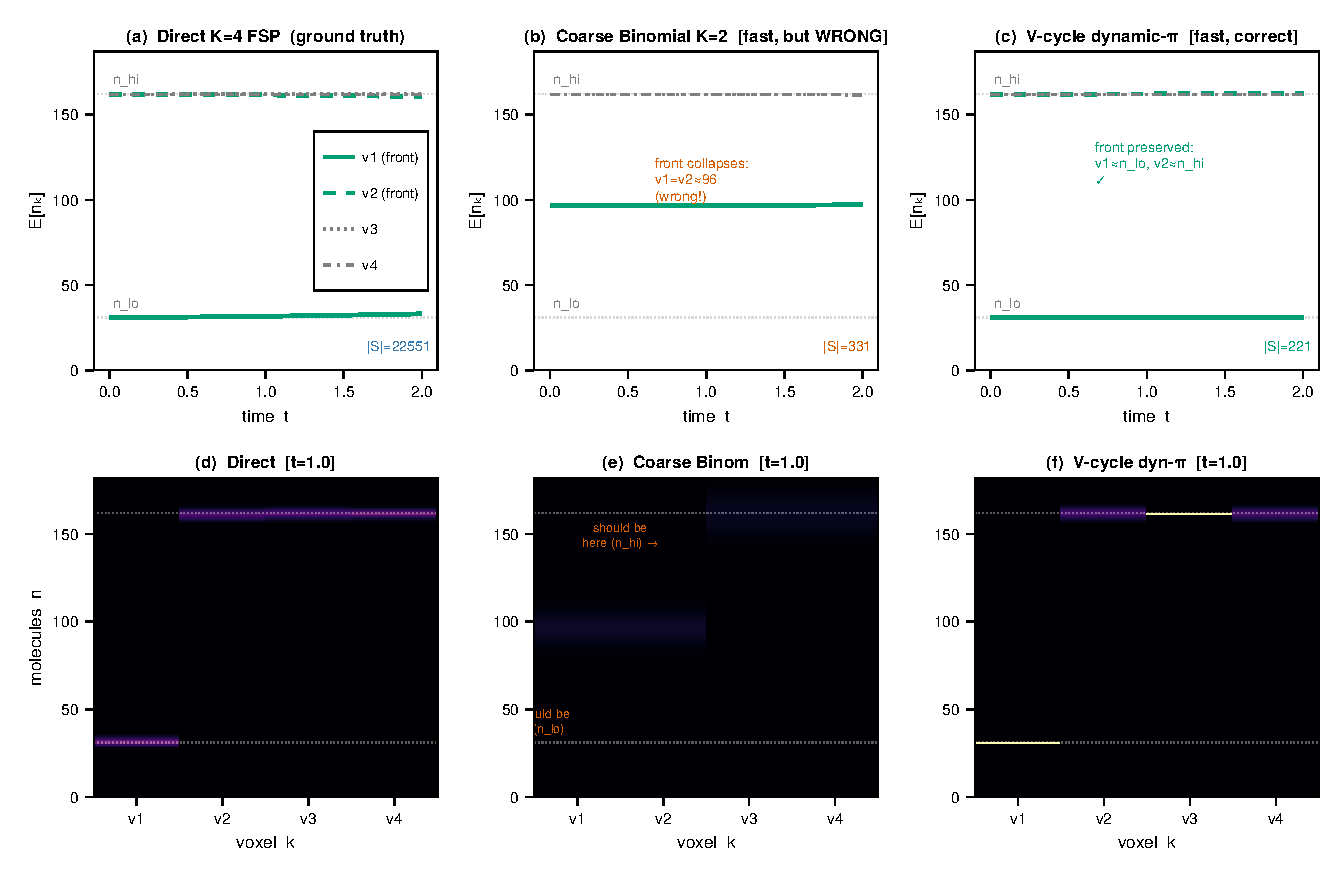
\includegraphics[width=0.93\textwidth,keepaspectratio]{fig_talk_schlogl}
\end{center}
\vspace{-0.5em}
{\footnotesize
K=4 Schl\"{o}gl, IC\,=\,$(n_\text{lo},n_\text{hi},n_\text{hi},n_\text{hi})$, front in pair 1.\quad
\textbf{Top:} voxel means.
\textbf{(a)} Direct (22k states), ground truth.
\textbf{(b)} Coarse Binomial (331 states): front collapses to ${\approx}96$ (wrong).
\textbf{(c)} V-cycle dyn-$\pi$ (221 states): correct, same cost as coarse.
\textbf{Bottom:} spatial marginals at $t{=}1$ confirm (b) is wrong, (c) matches (a).}
\end{frame}

%================================================================
%  SUMMARY
%================================================================

\begin{frame}{Summary}

  \begin{block}{1.\quad Fast diffusion enables state-space compression.}
    When the joint distribution of two adjacent voxels is near $\Bin(\bar n,\tfrac12)$,
    replacing $(n_1,n_2)$ by $\bar n$ cuts the per-pair state space
    from $n_{\max}^{2S}$ to $n_{\max}^{S}$.
    \emph{K=8 birth-death wavefront solved with 30k states (direct: intractable).}
  \end{block}

  \smallskip
  \begin{block}{2.\quad Bistable fronts require dynamic-$\pi$ prolongation.}
    At a front, the within-pair distribution is bimodal: Binomial is wrong.
    The imbalance $\alpha_j$ detects this at runtime.
    V-cycle with dynamic-$\pi$ corrects the prolongation.
    \emph{K=4 Schl\"{o}gl: V-cycle 221 states, direct 22k, both accurate.}
  \end{block}

  \smallskip
  \begin{block}{3.\quad Same algorithm: $\alpha_j$ adapts automatically.}
    Birth-death: $\alpha_j{\approx}0$ always $\Rightarrow$ merge all pairs.
    Schl\"{o}gl: $\alpha_j{\approx}1$ at front $\Rightarrow$ keep fine.
    One algorithm handles both.
  \end{block}

  \smallskip
  \textbf{Open:} multi-level hierarchy; multi-species; moving fronts; rigorous error bounds.

\end{frame}

%================================================================
\appendix
%================================================================

\begin{frame}{Appendix: why not reconstruct at every step?}

  \begin{columns}[T]
    \begin{column}{0.50\textwidth}
      \begin{center}
      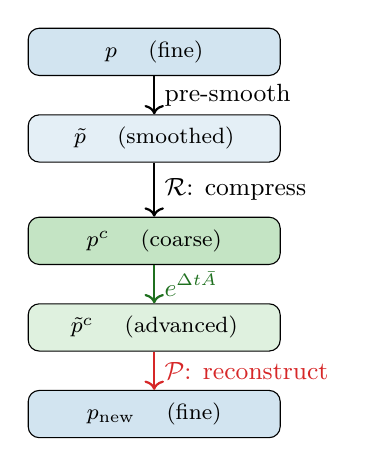
\begin{tikzpicture}[every node/.style={font=\footnotesize},scale=1.0]
        \node[draw,rounded corners,fill=myblue!20,
              minimum width=3.2cm,minimum height=0.6cm]
          (f1) at (0,4.6) {$p$ \quad (fine)};
        \node[draw,rounded corners,fill=myblue!12,
              minimum width=3.2cm,minimum height=0.6cm]
          (f2) at (0,3.5) {$\tilde p$ \quad (smoothed)};
        \node[draw,rounded corners,fill=coarsegreen!28,
              minimum width=3.2cm,minimum height=0.6cm]
          (c1) at (0,2.2) {$p^c$ \quad (coarse)};
        \node[draw,rounded corners,fill=coarsegreen!15,
              minimum width=3.2cm,minimum height=0.6cm]
          (c2) at (0,1.1) {$\tilde p^c$ \quad (advanced)};
        \node[draw,rounded corners,fill=myblue!20,
              minimum width=3.2cm,minimum height=0.6cm]
          (f3) at (0,0.0) {$p_{\rm new}$ \quad (fine)};
        \draw[->,thick] (f1.south)--(f2.north) node[midway,right]{\small pre-smooth};
        \draw[->,thick] (f2.south)--(c1.north) node[midway,right]{\small $\calR$: compress};
        \draw[->,thick,coarsegreen!70!black] (c1.south)--(c2.north) node[midway,right]{\small $e^{\Delta t \bar A}$};
        \draw[->,thick,slowred] (c2.south)--(f3.north) node[midway,right]{\small $\calP$: reconstruct};
      \end{tikzpicture}
      \end{center}
    \end{column}
    \begin{column}{0.46\textwidth}
      \begin{alertblock}{Reconstruction is wrong at the front}
        Step 4 forces a Binomial split on \emph{every} pair,
        including the front where the true distribution is bimodal.\\[0.5em]
        \textbf{Fix:} evolve $p^M$ directly: no reconstruction step.
        Coarse pairs carry the Binomial assumption implicitly in $\bar A_j$;
        the fine window tracks the true within-pair distribution exactly.
      \end{alertblock}
    \end{column}
  \end{columns}

\end{frame}

\begin{frame}{Appendix: mixed-resolution generator is self-consistent}
  \begin{center}
    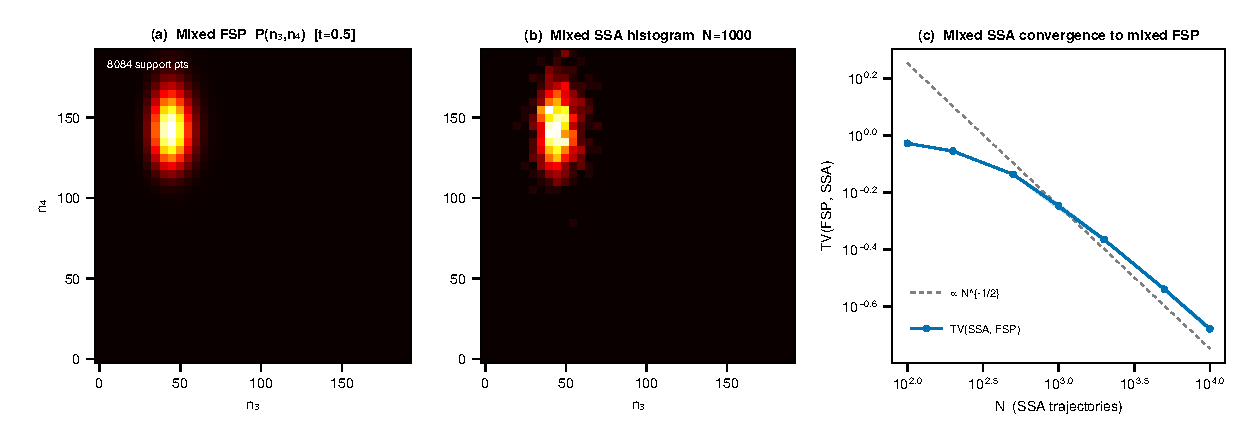
\includegraphics[width=0.78\textwidth,keepaspectratio]{fig_mixed_fsp_ssa}
  \end{center}
  {\footnotesize
    ODE solve on the mixed state $(\bar n_1, n_3, n_4)$
    vs.\ Monte Carlo on the same reduced generator.
    Means agree to ${<}1\%$; TV $\sim N^{-1/2}$ (sampling noise only).
  }
\end{frame}

\begin{frame}{Appendix: probability dynamics (birth-death vs.\ Schl\"{o}gl)}
\begin{center}
  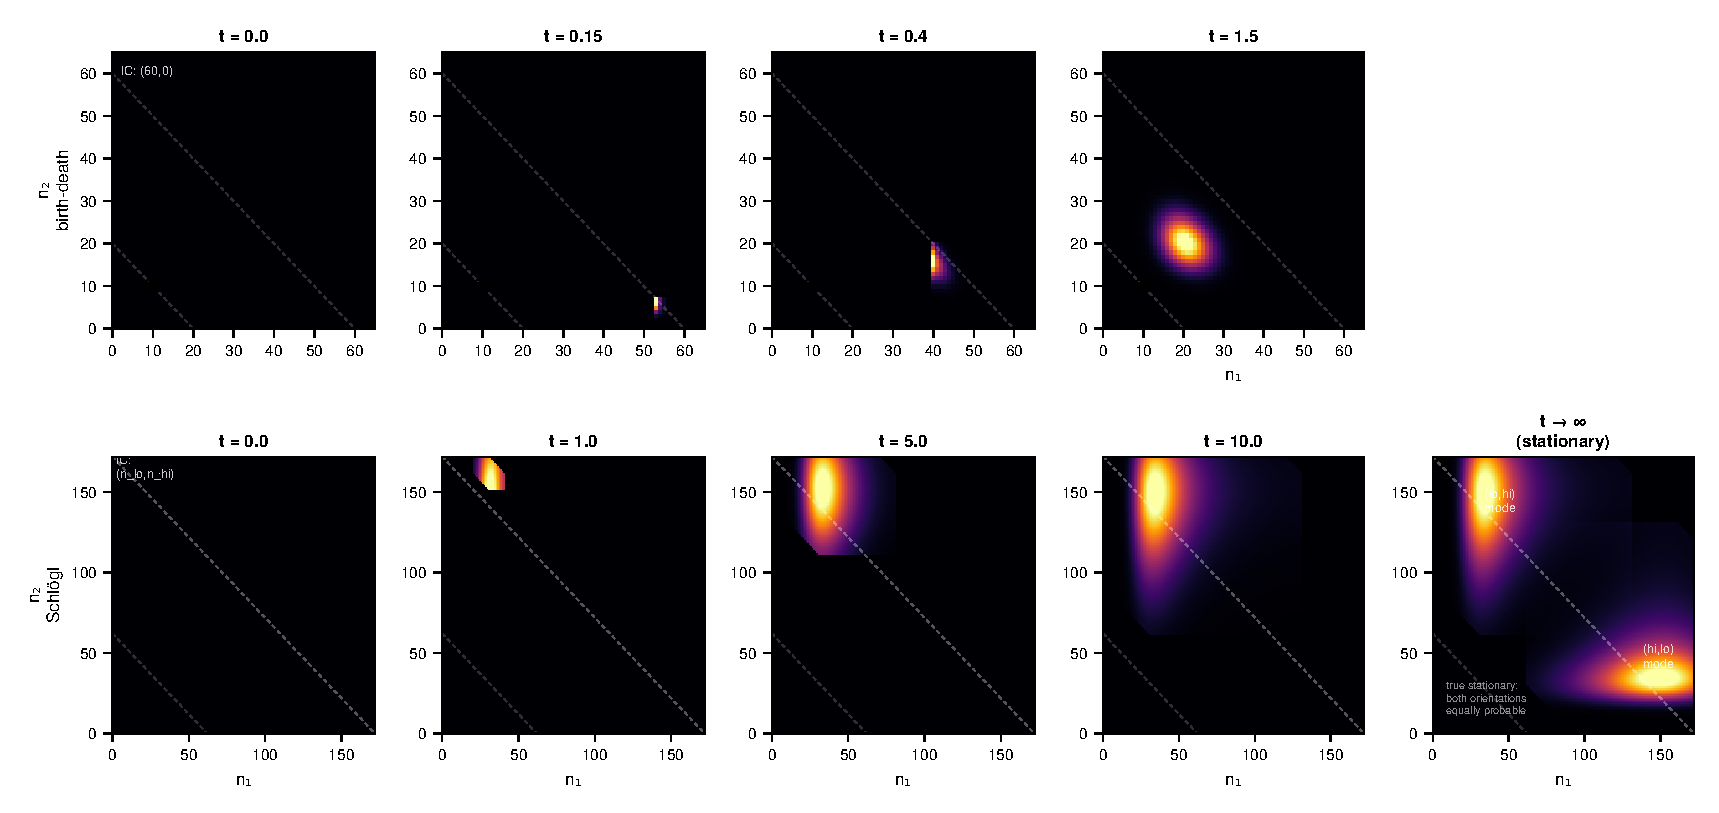
\includegraphics[width=0.92\textwidth,keepaspectratio]{fig_talk_diffusion}
\end{center}
{\footnotesize
\textbf{Top:} birth-death point source traveling to Poisson(10) stationary. Binomial coarsening exact.\\
\textbf{Bottom:} Schl\"{o}gl front IC persisting metastably; true stationary (rightmost) shows both orientations equally.}
\end{frame}

\begin{frame}{Appendix: K=8 persistent front (detailed)}
  \begin{center}
    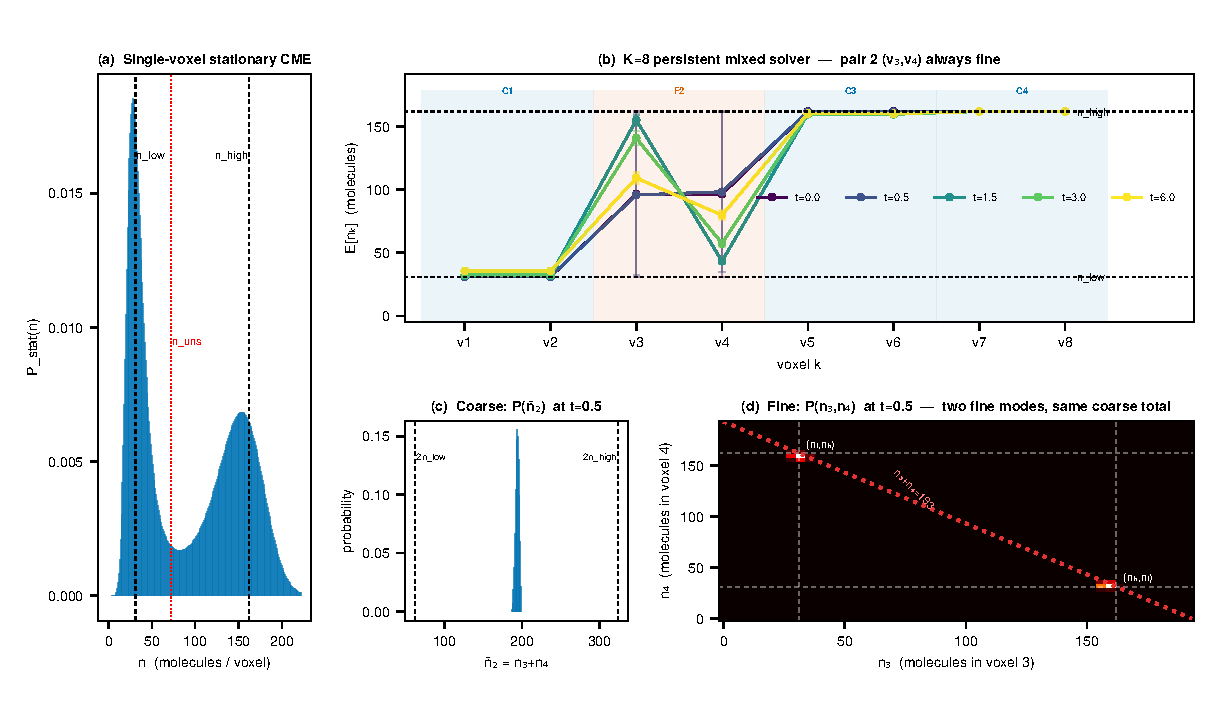
\includegraphics[width=0.82\textwidth,height=0.70\textheight,keepaspectratio]{fig_k8_persistent}
  \end{center}
\end{frame}

\begin{frame}{Appendix: K=12 persistent front}
  \begin{center}
    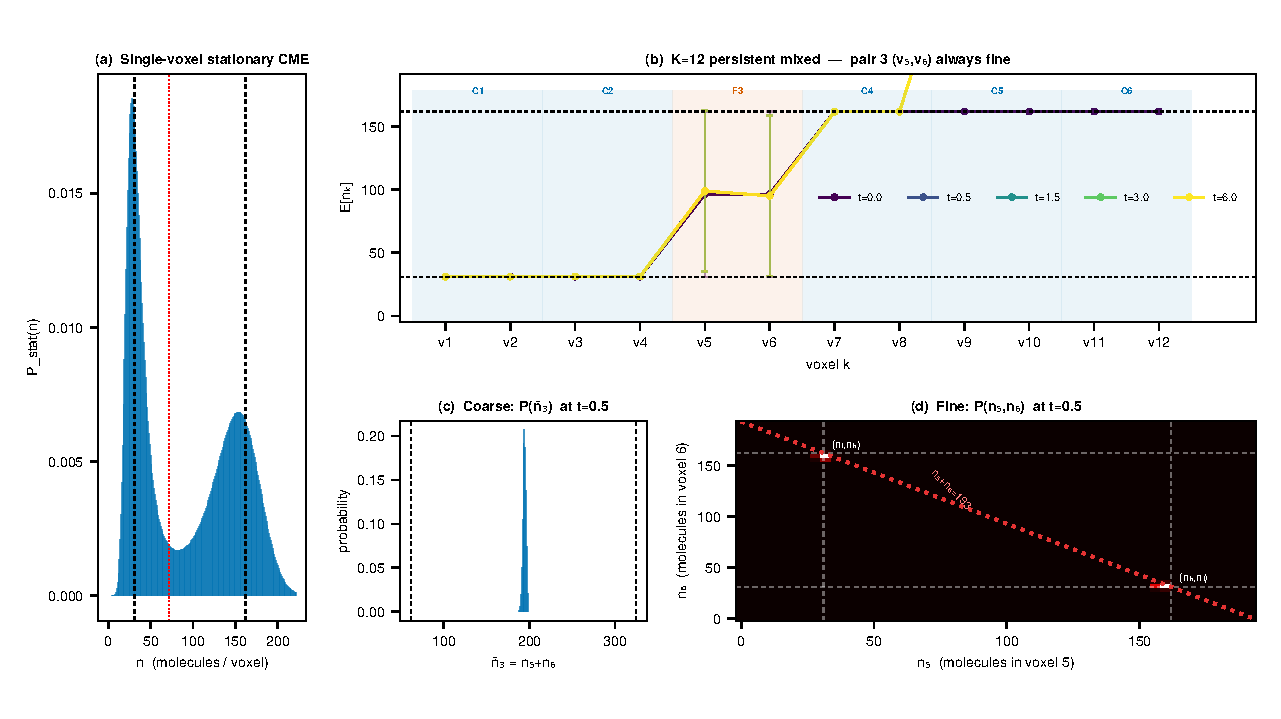
\includegraphics[width=0.80\textwidth,height=0.68\textheight,keepaspectratio]{fig_k12_persistent}
  \end{center}
\end{frame}

\end{document}
